\section{Solution}
\subsection{Idea}
In this section we describe the key ideas behind our design, and the decisions we made during the design process.

First we had to decide which design option of the 4 given options we were going to use. As seen in our answers to question 3 in section ~\ref{sec:Q3} a naive scaler is very inefficient; the naive direct scaler would require roughly all the resources of the entire Spartan FPGA to scale a single audio stream in real time. So we will implement the scaler using the direct equation. Now we have to decide between doing the scaling directly, or composing it of multiple scalers. The trade-off here is that a direct scaler has to store more coefficients on the board, whereas a composed scaler uses more multiplications per output. Also, for each scaler we introduce in a composed scaler the latency of the system is increased. As the number of coefficients turned out not to be a big problem, we decided to use one direct scaler from $44.1$ KHz to $48$ KHz.

The next choice we had to make was whether to optimize the scaler for resource usage or for throughput. We decided to optimize for throughput. The most important implication this choice has is that we will use 4 parallel multipliers for the FIR, instead of doing 4 sequential multiplications on one multiplier. We can now compose a diagram of the architecture of our system, figure ~\ref{fig:arch}. The coefficients are stored in read only memory (ROM), not visible in the diagram. Some additional hardware is required to get the right coefficient \texttt{h[i]} our of the ROM.

To generate the actual coefficients we wrote a small Java program (section ~\ref{sec:java}) that given some \texttt{L} generates all coefficients  in 16 bit signed hex notation. We scaled the coefficients such that they sum up to $(2^{15}-1)\cdot L$, this way the output signal will have the same intensity as the input signal.

\begin{figure}
\begin{center}
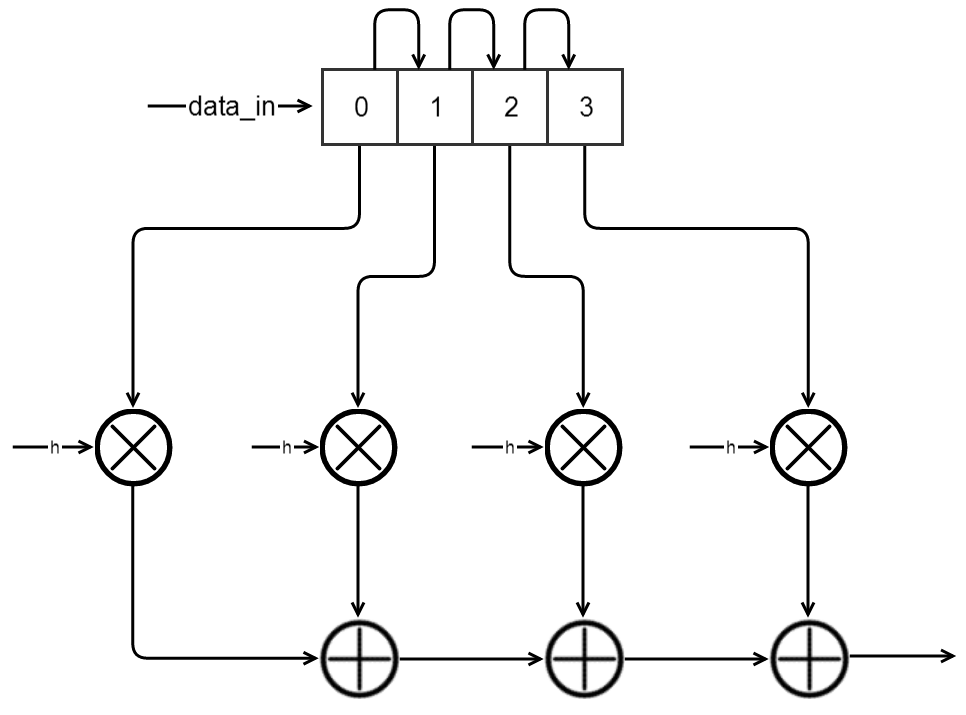
\includegraphics[width=0.7\textwidth]{images/architecture.png}
\caption{Architecture diagram of the scaler.}
\label{fig:arch}
\end{center}
\end{figure}

Another observation we made is that since the \texttt{lanczos2} function is symmetric, the coefficients are symmetric as well. So we optimized our program by only storing about half ($2L+1$ instead of $4L$ to be precise) of the coefficients. After implementing this optimization we noticed that as well as using fewer registers, the post PAR static timing report showed an increase in clock frequency. This is likely because the optimized version needs fewer wires which allows for more efficient routing.

\subsection{Implementation}
In this section we will explain functional correctness of our code. The Verilog source code of our filter can be found in section ~\ref{sec:source}. \\
\\
\centerline{reg [0:L\_LOG-1] l;}\\
\\
We use the direct equation, this register store the value of $nM \bmod L$, so we can calculate it using only conditionals and adders.\\
\\
\centerline{reg signed [0:DWIDTH-1] in [0:3];}\\
\\
For the direct equation we need to store the 4 most recent input values.\\
\\
\centerline{reg signed [0:DWIDTH-1] h [0:2*L];}\\
\\
We need to store our coefficients. As explained in the previous section, the coefficients are symmetric. So we can do an optimization storing only $2L + 1$ coefficients.\\
\\
\centerline{reg signed [0:DDWIDTH-1] partial1;}\\
\centerline{reg signed [0:DDWIDTH-1] partial2;}\\
\centerline{reg signed [0:DDWIDTH-1] partial3;}\\
\centerline{reg signed [0:DDWIDTH-1] partial4;}\\
\\
We pipelined the system by adding a delay between each of the 4 multiplier and the accumulator of the FIR, this increases throughput.\\
\\
\centerline{\$readmemh("coefficients.txt", h);}\\
\\
Our coefficients are read from a file. These values are precalculated by a small Java program.\\
\begin{center}
\parbox{10cm}{
in[0] $<=$ data\_in;\\
in[1] $<=$ in[0];\\
in[2] $<=$ in[1];\\
in[3] $<=$ in[2];\\
req\_in\_buf $<=$ 0;\\
}
\end{center}
As seen in figure ~\ref{fig:arch}, all values in the input buffer are shifted, the new input is loaded into the first.\\
\begin{center}
\parbox{10cm}{
if( l $<$ L - M )\\
begin\\
\phantom{xxxx} l $<=$ l + M;\\
end\\
else\\
begin\\
\phantom{xxxx}l $<=$ l - (L - M);\\
\phantom{xxxx}req\_in\_buf $<=$ 1;\\
end\\
}
\end{center}
This is used to efficiently calculate the value of $(l + M) \bmod L$. Instead of applying the $\bmod$ operation each time, we store the value, and increment in by $l + M$. When this value becomes larger or equal to  $L - M$ we have to subtract $L - M$.\\
\begin{center}
\parbox{10cm}{
partial1 $<=$ in[0] * h[l];      // h[l+L*0] \\
partial2 $<=$ in[1] * h[l+L];    // h[l+L*1]\\
partial3 $<=$ in[2] * h[L*2-l];  // h[l+L*2], mirrored\\
partial4 $<=$ in[3] * h[L-l];    // h[l+L*3], mirrored\\
sum $<=$ partial1 + partial2 + partial3 + partial4;\\
}
\end{center}
This is the filtering part, the multiplications and additions are done in separately because we pipelined the system by buffering between them.

\centerline{}
